\documentclass[letter]{beamer}
\usepackage{mathtools}
\usepackage{pgfplotstable}%for generating latex from csv files
\usepackage{datetime}
\usepackage{hyperref}


\title{``A New Series Representation for Time Invariant Functions and
a Solution Strategy for Occasionally Binding Constraints in Rational Expectations Models''}
\date{\currenttime -- \today }



\author{Gary S. Anderson\thanks{Note that these slides will likely be updated daily till November 19th. I would like to thank Luca Guerrieri, Christopher Gust and Robert Tetlow for their comments and suggestions. }}
\newcommand{\xtFuncTI}{\mathcal{X}(x,\epsilon)}
\newcommand{\XtFuncTI}{\mathbf{X}(x)}

\newcommand{\xtFunc}[1]{\mathcal{X}{#1}}
\newcommand{\XtFunc}[1]{\mathbf{X}{#1}}



\newcommand{\discr}[1]{\mathcal{D}^{#1}(x_{t-1},\epsilon_t)}

\newcommand{\XZPair}[1]{(\mathcal{X}^{#1},\mathcal{Z}^{#1})}
\newcommand{\XZPairG}[1]{(\mathcal{X}^{#1}(x^g),\mathcal{Z}^{#1}(x^g))}
\newcommand{\xIter}[2]{\mathcal{X}^{#1}(#2)}
%\newcommand{\zNow}[1]{z^{#1}_0(x_{t-1},\epsilon_t)}
%\newcommand{\ZNow}[3]{\mathcal{Z}^{#1}_{#2}(x_{#3})}
\newcommand{\zNow}[1]{z^{#1}(x_{t-1},\epsilon_t)}
\newcommand{\ZNow}[3]{\mathcal{Z}^{#1}(x_{#3})}

\newcommand{\xNow}[1]{x^{#1}_t(x_{t-1},\epsilon_t)}
\newcommand{\xNowtp}[1]{x^{#1}_{t+1}(x_{t-1},\epsilon_t)}
\newcommand{\XNow}[3]{\mathcal{X}^{#1}_{#2}(x_{#3})}








\newcommand{\sForSum}{{\nu}}
\newcommand{\rcpC}{{\mathbf{c}}}

\newcommand{\xtVec}{  \begin{bmatrix}
    q_t\\r_{t}\\r_{ut}
  \end{bmatrix}
}
\newcommand{\xtPVec}{  \begin{bmatrix}
    q_{t+1}\\r_{t+1}\\r_{ut+1}
  \end{bmatrix}
}
\newcommand{\xtMVec}{  \begin{bmatrix}
    q_{t-1}\\r_{t-1}\\r_{ut-1}
  \end{bmatrix}
}
\newcommand{\expctEps}[1]{\mathcal{E}_{\epsilon} \left [#1 \right ]}
\newcommand{\expct}[2]{E_{#1} \left [#2 \right ]}
\newcommand{\expc}[1]{\mathcal{E} \left [#1 \right ]}
\newcommand{\expcK}[2]{\mathcal{E}^{#1} \left [#2 \right ]}
\newcommand{\xsln}[1]{\mathbb{X} \left [#1 \right ]}
\newcommand{\xslnK}[2]{\hat{\mathbb{X}}^{#1} \left [#2 \right ]}
\newcommand{\xpth}[2]{\mathfrak{X}_{#1} \left [#2 \right ]}
\newcommand\infNorm[1]{\left\lVert#1\right\rVert_\infty}
\newcommand\twoNorm[1]{\left\lVert#1\right\rVert_2}
%\newcommand{\inorm}[1]{\left\lVert#1\right\rVert_\infty}

% \newcommand{\forPhi}{\begin{bmatrix}
% \psi_\epsilon&\psi_z
% \end{bmatrix}}
% \newcommand{\phiMult}{\phi \psi_\epsilon}
% \newcommand{\bMult}{B x_{-1} + \phiMult}
\newcommand{\phiMultBoth}[1]{
	\phi (\psi_\epsilon \epsilon_t +\psi_z z_0^#1(x_{-1},\epsilon_t))}
\newcommand{\bMultBoth}[1]{B x_{-1} + \phiMultBoth{#1}}


\newcommand{\bForOne}{\bMultBoth{1}
}

% \newcommand{\bForTwo}{\bMultBoth{2}+
% F \phi  \psi_z  
% Z_0^1(x_0^2(x_{-1}))   
% }



\newcommand{\compSlack}{z_0^1(x_{-1},\epsilon_t) \left ( \bar{x} -x\right )=0\\ z_0^1(x_{-1},\epsilon_t)> 0}
% \begin{gather*}
% 0= x_t-(B x_{t-1}+ \phi \psi_\epsilon\epsilon_t + \phi \psi_z 
% \xpt{z_{t}(x_{t-1},\epsilon_t)    } )
% \end{gather*}

\newcommand{\xpt}[1]{#1}


\makeatletter
\@ifundefined{newblock}{%
 \def\newblock{\hskip .11em plus .33em minus .07em} % important line
}
\makeatother


\makeatletter
\pgfplotsset{
    /pgfplots/table/omit header/.style={%
        /pgfplots/table/typeset cell/.append code={%
            \ifnum\c@pgfplotstable@rowindex=-1
                \pgfkeyslet{/pgfplots/table/@cell content}\pgfutil@empty%
            \fi
        }
    }
}
\makeatother
 

\makeatletter
\newcommand*\ExpandableInput[1]{\@@input#1 }
\makeatother


\newcommand{\tpExp}[1]{\phi^e_{#1}(x_{t-1})}
\newcommand{\lRat}[2]{\log \left( \frac{z_{#1}}{z_{#2}}\right)}


\newcommand{\anEdit}[1]
{

{\color{blue}
\begin{quote}
#1  
\end{quote}}

}

\mathtoolsset{showonlyrefs}
\usepackage{pseudocode}

\begin{document}


\begin{frame}
  \titlepage
\end{frame}



\begin{frame}
  \frametitle{Context and Motivation}
  \begin{itemize}
  \item Why bother with all this math/computing stuff?
  \item Non linear models in general more important 
  \item Modeling Occasionally Binding Constraints (OBC) increasingly important
  \item Useful to have  a coherent framework for attacking a variety of complicated models 
  \item Specific Authors and Examples...

  \end{itemize}
\end{frame}



\begin{frame}
  \frametitle{Overview}
  \begin{itemize}
  \item  new representation for time invariant functions.
  \item  series representation broadly applicable for nonlinear rational expectations models 
\item  formula for accuracy bounds for any 
proposed time invariant model solution.
\item an important component in an algorithm for constructing approximate solutions 
\item facilitates exploiting the ``law of iterated expectations'' in computing solutions for models with occasionally binding constraints.
\item Mathematica code implementing the algorithms
  \end{itemize}
\end{frame}

\begin{frame}
\frametitle{Models to Approximations }
  \begin{gather}
    \fbox{Nonlinear Rational Expectations Model}\\ \Downarrow\\
\fbox{Bounded Time Invariant Function Solution}\\\Downarrow\\
\fbox{Series Representation}\\\Downarrow\\
\fbox{Series Approximation}
  \end{gather}
  \begin{itemize}
  \item  How can we take the  steps?
  \item  How can we skip the intermediate steps?
  \end{itemize}

\end{frame}
\begin{frame}
  \frametitle{Time Invariant Functions}

Consider a time invariant stochastic function $\xtFuncTI$, 
\begin{itemize}
\item where $x$ is an $L$ dimensional real variable
\item $\epsilon$ a $K$ dimensional random variable.
\item time $t$ realizations of $\epsilon$, $\epsilon_t$, are independently and identically distributed.
\end{itemize}
We define a time invariant deterministic function $\XtFuncTI\equiv \expctEps{\xtFuncTI}$ and denote
\begin{gather*}
\expct{t}{x_{t+k}}\equiv\begin{cases}
\xtFunc{(x_{t-1},\epsilon_t)} &k=0\\
\XtFunc{(\expct{t}{x_{t+k-1}})} &k>0
\end{cases}
\end{gather*}

\end{frame}

\begin{frame}
  \frametitle{Iterating Forward: Conditional Expectations}
Consider Iterating the function $\mathcal{X}$ forward by 
recursively applying $\mathcal{X}$ to compute a solution path
\begin{gather}
\underbrace{(x_{t-1},\epsilon_t)} 
\underbrace{{\mathcal{X}}(x_{t-1},\epsilon_t)}
\underbrace{\int {\mathcal{X}}({\mathcal{X}}(x_{t-1},\epsilon_t),\epsilon_{t+1})}
\underbrace{\ldots}
\intertext{Suppose this process produces bounded trajectories for $\mathcal{X}$}
   \mathcal{X}_{t+s}(x_{t-1},\epsilon_t), \,\,\mathcal{X}_{t+s} \in{R^k}\,\,\infNorm{\mathcal{X}_{t+s}}  \le \bar{\mathcal{X}}\,\,\forall s\ge 0 \label{fFamily}.
 \end{gather}

 \begin{itemize}
 \item It will then be possible to write down a useful 
series representation for
the function $\mathcal{X}(x_{t-1},\epsilon_t)$.
\item Based on discrepancies from some ``arbitrary'' Blanchard-Kahn linear dynamic system
 \end{itemize}

 % \begin{itemize}
 % \item Law of Iterated Expectations applies
 %   \begin{gather*}
 %     E_t(\mathcal{X}(x_{t+k-1},\epsilon_{t+k}))=
 %     E_t(E_{t+k}(\mathcal{X}(x_{t+k-1},\epsilon_{t+k})))
 %   \end{gather*}
 % \end{itemize}


\end{frame}


\begin{frame}
  \frametitle{Series Representation}
  \begin{itemize}
  \item 
For any linear homogeneous 
$k$ dimensional 
deterministic 
system, 
\begin{gather}
  	 H_{-1} x_{t-1} + H_0 x_t + H_1 x_{t+1}=0\label{hSystem}
\end{gather}
\item that produces  a unique stable solution, 
it is well known\ \cite{anderson10} that
  

\begin{gather}
	 H_{-1} x_{t-1} + H_0 x_t + H_1 x_{t+1}=\psi_\epsilon \epsilon_t +\psi_{c}
\intertext{as}
x_t=B x_{t-1} + \phi \psi_\epsilon \epsilon_t + (I - F)^{-1} \phi \psi_c
\intertext{where}
\phi= (H_0 +H_1 B)^{-1} %\\F=-\phi H_1 
\end{gather}
\item 
Define $\linMod \equiv \linModMats$
  \end{itemize}

\end{frame}


\begin{frame}
  \frametitle{Series Representation}
{\small
Given the trajectories \refeq{fFamily}, define 
$  z_{t+s}(x_{t-1},\epsilon_t)$ as  %\footnote{These $z$ functions will soon prove useful in an algorithm for computing unknown trajectories like \refeq{fFamily}.}:
{

  \begin{align}
  z_{t+s}(x_{t-1},\epsilon_t) \equiv& H_{-1} \mathcal{X}_{t-1}(x_{t+s-1},\epsilon_t) + \nonumber\\
& H_0 \mathcal{X}_{t+s}(x_{t-1},\epsilon_t) +  \label{defZ} \\
& H_1 \mathcal{X}_{t+s+1}(x_{t-1},\epsilon_t) \nonumber
  \end{align}
}


\cite{anderson10}  demonstrates that, for 
such models,
	 \begin{gather}
	 \mathcal{X}_{t}(x_{t-1},\epsilon_t) =B x_{t-1}+ \phi \psi_\epsilon\epsilon_t + \sum_{\sForSum=0}^\infty F^s \phi z_{t+\sForSum}(x_{t-1},\epsilon_t) + (I - F)^{-1} \phi \psi_c
\label{theSeries}\intertext{and}
	 \mathcal{X}_{t+s+1}(x_{t-1},\epsilon_t) =B \mathcal{X}_{t+s} + \sum_{\sForSum =0}^\infty F^\sForSum \phi z_{t+s+\sForSum}(x_{t-1},\epsilon_t) + (I - F)^{-1} \phi \psi_c \,\,\,\forall s \ge  0
\intertext{where}
F=-\phi H_1 
	 \end{gather}
}

\end{frame}


\begin{frame}
  \frametitle{RBC Model Example}
  
\begin{gather}
\frac{1}{c_t^{\eta}}=\alpha \delta k_{t}^{\alpha-1} E_t \left (\frac{\theta_{t}}{c_{t+1}^\eta} \right ) \\
c_t + k_t=\theta_{t-1}k_{t-1}^\alpha \\
\ln \theta_t =\rho \ln \theta_{t-1} + \epsilon_t\label{rbcSys}
\intertext{for $\eta=1$}
\frac{1}{c_t}=\alpha \delta k_{t}^{\alpha-1} E_t \left (\frac{\theta_{t}}{c_{t+1}} \right ) \\
c_t + k_t=\theta_{t-1}k_{t-1}^\alpha \\
\ln \theta_t =\rho \ln \theta_{t-1} + \epsilon_t\label{rbcSys}
\intertext{and there is a closed form solution}
  k_{t}= \theta_{t-1} \alpha \delta k_{t-1}^\alpha.\label{soln}\\
c_t= \theta_{t-1} k_{t-1}^\alpha (1-\alpha \delta) 
\end{gather}
\end{frame}

\begin{frame}
  \frametitle{An ``Almost Arbitrary'' Linear Model}
 {\small 
Consider the following constructed from ``nearly'' arbitrary coefficients
\begin{gather}
  \begin{bmatrix}
H_{-1}&H_{0}&H_{1} 
  \end{bmatrix}=
\vcenter{\hbox{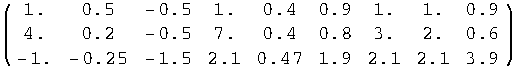
\includegraphics{refHmat.pdf}}}\intertext{with $\psi_c=\psi_\epsilon=0, \,\,  \psi_z=I$.
These coefficients  happen to produce a unique stable solution.}
  B=
\vcenter{\hbox{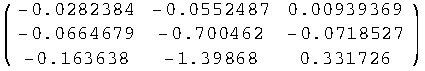
\includegraphics{refBmat.pdf}}}\\
\phi=
\vcenter{\hbox{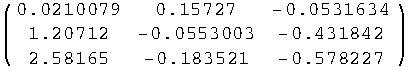
\includegraphics{refPhimat.pdf}}}\\
F=
\vcenter{\hbox{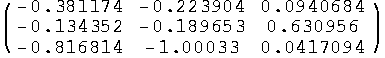
\includegraphics{refFmat.pdf}}}
\end{gather} 
}
\end{frame}




\begin{frame}
  \frametitle{Series Approximation Truncation Errors}
  \begin{itemize}
  \item Can choose an ``arbitrary''  linear system unrelated (save for dimensionality) to origin of the solution trajectories
  \item can choose the number of series terms
    \begin{gather}
      \label{eq:1}
\sum_{s=k+1}^{\infty} F^s \phi \psi_z = (I -F)^{-1} F^{k+1}\phi \psi_z       
    \end{gather}
  \item More terms more accuracy
  \item linear system with more ``similar'' dynamics more accuracy for given number of terms
  \item RBC example
    \begin{itemize}
    \item ``arbitrary'' linear system

\framebox{Table will show truncation errors for the ``Arbitrary'' Linear Model}
  \item linearized RBC  linear system

\framebox{Table will show truncation errors for the  Linearized RBC Model}
    \end{itemize}

  \end{itemize}
\end{frame}
\begin{frame}
  \frametitle{Assessing Rational Expectations Solution Accuracy}
{\small
  \begin{itemize}
  \item Use auxiliary variables for nonlinear stochastic ``chunks''
  \item the $m$ function codifies changes in model equations due to
inequality constraints or regime switching.$(\varpi \in \{1,\ldots,n\})$
\item interested in finding a time invariant function $g^\ast$ that satisfies
 \begin{gather}
   \begin{split}
 h_{\varpi}(x_{t+s-1},g^\ast(x_{t+s-1},\epsilon_{t+s}),\mathcal{H}[g^\ast(g^\ast(x_{t+s-1},\epsilon_{t+s}),\epsilon_{t+s+1})],\epsilon_{t+s}) \label{theProblem} \\
\varpi= m(x_{t+s-1},g^\ast(x_{t+s-1},\epsilon_{t+s}),\mathcal{H}[g^\ast(g^\ast(x_{t+s-},\epsilon_{t+s}),\epsilon_{t+s+1})],\epsilon_{t+s}) 
   \end{split}\intertext{ for all $s>0$ where $\mathcal{H}$ is an operator,    that maps stochastic to deterministic functions}
  \end{gather}
 \begin{description}
 \item[Perfect Foresight]
 \begin{gather}
      \mathcal{H}^{PF}[g^{k}(x,\epsilon_{t+T-k+1})]=
 g^{k}(x,0)\\
 \end{gather}
 \item[Rational Expectations] 
 \begin{gather}
      \mathcal{H}^{RE}[g^{k}(x,\epsilon_{t+T-k+1})]=
 \mathcal{E}_t[g^{k}(x,\epsilon_{t+T-k+1})|x]\\
 \end{gather}
 \end{description}
  \end{itemize}
}  
%  \intertext{define} 
%  \mathcal{G}^\ast(x_{t+s-1},\epsilon_{t+s})= \mathcal{H}[g^\ast(g^\ast(x_{t+s-1},\epsilon_{t+s}),\epsilon_{t+s+1})] \nonumber


\end{frame}

\begin{frame}
  \frametitle{Assessing Accuracy}
{\small

  \begin{itemize}
  \item As with series approximation,
 construct a family of bounded trajectories and compute
$  z_{t+s}(x_{t-1},\epsilon_t)$ as  %\footnote{These $z$ functions will soon prove useful in an algorithm for computing unknown trajectories like \refeq{fFamily}.}:
{
\begin{gather}
  z_{t+s}(x_{t-1},\epsilon_t) \equiv\\
   \begin{split}
 h_{\varpi}(\mathcal{X}_{t+s-1},g^\ast(\mathcal{X}_{t+s-1},\epsilon_{t+s}),\mathcal{H}[g^\ast(g^\ast(\mathcal{X}_{t+s-1},\epsilon_{t+s}),\epsilon_{t+s+1})],\epsilon_{t+s}) \label{theProblem} \\
\varpi= m(\mathcal{X}_{t+s-1},g^\ast(\mathcal{X}_{t+s-1},\epsilon_{t+s}),\mathcal{H}[g^\ast(g^\ast(\mathcal{X}_{t+s-},\epsilon_{t+s}),\epsilon_{t+s+1})],\epsilon_{t+s}) 
   \end{split}
  \end{gather}
}
\item The formula provides information about how much $x_{t}$ would need
to change in order for the trajectory to honor the constraints along the path
\item An exact solution would produce zero for all the $z$ functions
\item One can use a truncated series to carry out the approximation for changes in $x_t$
  \end{itemize}
}
\end{frame}

\begin{frame}
  \frametitle{Assessing Accuracy: the RBC Model Example}
  \begin{itemize}
  \item Validate the exact solution

\framebox{``Arbitrary'' Linear Model} =\framebox{linearized RBC Linear Model}
  \item How close is the perfect foresight solution to $\eta=1$ solution
\framebox{Table of truncation errors ``Arbitrary'' Linear Model} $\ne$\framebox{table of truncation errors linearized RBC Linear Model}
  \item How close is the perfect foresight solution to $\eta \ne 1$ solution
\framebox{Table of truncation errors ``Arbitrary'' Linear Model} $\ne$\framebox{table of truncation errors linearized RBC Linear Model}
  \item How close is the exact $\eta=1$  solution to $\eta \ne 1$ solution
\framebox{Table of truncation errors ``Arbitrary'' Linear Model} $\ne$\framebox{table of truncation errors linearized RBC Linear Model}
  \end{itemize}
\end{frame}

\begin{frame}
  \frametitle{Correctly Computing Expectations of Nonlinear Functions}

  \begin{itemize}
  \item Formula maps future equation errors in to current time changes in model
variables.
\item In what follows, $\epsilon_t$ is known so that,
given a function characterizing future expectation,  model requires
a deterministic solution at time $t$
\item The formula is linear in the potentially nonlinear $z$ functions
\item Auxiliary equations for non linear ``chunks'' provide mechanism for characterizing  nonlinear expectations in the future
  \end{itemize}
\end{frame}


\begin{frame}
  \frametitle{Correctly Computing Expectations of Nonlinear Functions}
{\small 
  \begin{itemize}
  \item solutions for models that can be written in  the form
\begin{gather}
  h_i(x_{t-1},x_{t},x_{t+1},\epsilon_t)=h^{det}_{io}(x_{t-1},x_{t},\epsilon_t)+\\ 
\sum_{j=1}^{p_i} [h^{det}_{ij}(x_{t-1},x_{t},\epsilon_t)h^{nondet}_{ij}(x_{t+1})]=0
\end{gather}
\item Euler equations for the  neoclassical growth  model 
\label{sec:simple-rbc-model-ext} 
\begin{gather}
h_{10}^{det}(\cdot)=\frac{1}{c_t^\eta},\,\,
h_{11}^{det}()=\alpha \delta \theta_{t}k_{t}^{\alpha-1} ,\,\,
h_{11}^{nondet}(\cdot)=E_t \left (\frac{1}{c_{t+1}^\eta} \right )\\
h_{20}^{det}(\cdot)=c_t + k_t-\theta_{t-1}k_{t-1}^\alpha,\,\,
h_{21}^{det}(\cdot)=0\\
h_{30}^{det}(\cdot)=\ln \theta_t -(\rho \ln \theta_{t-1} + \epsilon_t),\,\,
h_{31}^{det}(\cdot)=0
\end{gather}
\item $\epsilon_t$ is known, all stochastic components have $t+1$ time subscripts . 
\item include auxiliary variables for each $h_{ij}^{nondet}$  -- text assumes models orignally given in this form
  \end{itemize}

% the conditional expectation of nonlinear expressions,  
% accurately recursively computing  the appropriate expected values.
% Below, we will consider 
% systems that augment these dynamic equations with additional constraints 
% on the evolution of the variables.



}
\end{frame}




\begin{frame}
  \frametitle{Discovering Unknown Solutions}

A, conceptually, very simple solution strategy:  

  \begin{enumerate}
  \item Begin with some convergent linear model, $\linMod$, of appropriate dimension.
  \item Compute solutions valid for time t, 
but that assume the trajectories evolve according to the convergent linear model.
  \item Given solutions valid for time $t$ to $t+k$, extend the solutions to be valid for time $t$ to $t+k+1$ \label{stepNo}
\item Repeat step \ref{stepNo} unless truncation formulas indicate the solution is sufficiently accurate
  \end{enumerate}


\end{frame}

\begin{frame}
  \frametitle{The RBC Model ($\eta=1$): Recovering a Known Solution}
  \begin{itemize}
  \item Compute $\linMod$ for RBC Model $\eta=1,\rcpC_t=\frac{1}{c_t}$
  \end{itemize}

Applying formula \refeq{theSeries} produces:

{\tiny
\begin{gather}
  \begin{bmatrix}
c_t\\k_t\\ \rcpC_t\\\theta_t
  \end{bmatrix}=\\%paperCalcsRBCExample xt00
   \left(
   \begin{array}{c}
 0.359845 \epsilon _t+0.692632 k_{t-1}+0.341853 \theta _{t-1}-0.0442851
   \text{z1}_{t-1}+0.658 \text{z2}_{t-1}+0.359845 \text{z3}_{t-1}-0.111552 \\
 0.187032 \epsilon _t+0.36 k_{t-1}+0.17768 \theta _{t-1}+0.0442851
   \text{z1}_{t-1}+0.342 \text{z2}_{t-1}+0.187032 \text{z3}_{t-1}-0.0579799 \\
 -5.34898 k_{t-1}+0.342 \text{z1}_{t-1}-5.08153
   \text{z2}_{t-1}+\text{z4}_{t-1}+3.7794 \\
 \epsilon _t+0.95 \theta _{t-1}+\text{z3}_{t-1}+0.05 \\
   \end{array}
   \right)
\end{gather}
}

and 


{\tiny
%xt01=Private`computeNextXt[{Private`bmat,Private`phimat,Private`fmat,Private`psieps,Private`psic,Private`psiz},solnFunc00PF[[3+Range[3]]],{{cc},{kk},{tt}},{1}]//N//Expand//Simplify
\begin{gather}
  \begin{bmatrix}
c_{t+1}\\k_{t+1}\\ \rcpC_{t+1}\\\theta_{t+1}
  \end{bmatrix}=\\%paperCalcsRBCExample xt00
  \left(
   \begin{array}{c}
 0.471397 \epsilon _t+0.249347 k_{t-1}+0.447827 \theta _{t-1}+0.0306732
   \text{z1}_{t-1}+0.23688 \text{z2}_{t-1}+0.471397 \text{z3}_{t-1}-0.134618 \\
 0.245012 \epsilon_t+0.1296 k_{t-1}+0.232761 \theta _{t-1}+0.0159426
   \text{z1}_{t-1}+0.12312 \text{z2}_{t-1}+0.245012 \text{z3}_{t-1}-0.0699687 \\
 -1.00043 \epsilon _t-1.92563 k_{t-1}-0.950409 \theta _{t-1}-0.23688
   \text{z1}_{t-1}-1.82935 \text{z2}_{t-1}-1.00043 \text{z3}_{t-1}+4.08954 \\
 0.95 \epsilon _t+0.9025 \theta _{t-1}+0.95 \text{z3}_{t-1}+0.0975 \\
   \end{array}
   \right)
\end{gather}}


\end{frame}
\begin{frame}
  \frametitle{Begin by Solving a Deterministic System at time $t$}
{\small

  \begin{itemize}
  \item For any given $\left (  \begin{bmatrix}
c_{t-1}\\k_{t-1}\\ \rcpC_{t-1}\\\theta_{t-1}
  \end{bmatrix}, \epsilon_t \right )=\tArg$ 
compute
  \begin{gather}
    \label{eq:3}
    x_t^1\tArg=B x_{t-1} + \phi \psi_e\epsilon_t + \phi z^1_t\tArg\\
    E_t(x^1_{t+1}\tArg)=B x^1_{t}\tArg
  \end{gather}
\item The model equations provide a deterministic system  for computing $  z^1_t=\begin{bmatrix}
    z^1_{1t}\tArg\\
    z^1_{2t}\tArg\\
    z^1_{3t}\tArg\\
    z^1_{4t}\tArg
  \end{bmatrix}$.
\item The solution satisfies the nonlinear model equations for one 
period and the stand-in linear model for subsequent periods.
\item Assess accuracy
  \end{itemize}
}

\end{frame}

\begin{frame}
  \frametitle{Assess One Period Solution Accuracy}
  \begin{itemize}
  \item Show graphs of solution
  \item Show graphs of error
  \item Report accuracy assessment bounds
  \end{itemize}
\end{frame}

\begin{frame}
  \frametitle{Nonlinear 2 Periods: Solve time $t$ Deterministic
    System }
{\small
  \begin{itemize}
  \item Compute $Z^1(x)= E_t(z^1_t(x,\epsilon_t))$
  \item For any given $\tArg$ 
compute
{\small
  \begin{gather}
    x_t^2\tArg=B x_{t-1} + \phi \psi_e\epsilon_t + \phi z^2_t\tArg + F \phi Z^1(x^2_t) \label{bothS}\\
    E_t(x^2_{t+1}\tArg)=B x^2_{t}\tArg+ \phi Z^1(x^2_t)
  \end{gather}
}
\item The model equations provide a deterministic system  for computing $  z^2_t=\begin{bmatrix}
    z^2_{1t}\tArg\\
    z^2_{2t}\tArg\\
    z^2_{3t}\tArg\\
    z^2_{4t}\tArg
  \end{bmatrix}$.
\item The solution satisfies the nonlinear model equations for two 
period and the stand-in linear model for subsequent periods.
\item unlike the first step, $x^2_t$ appears on both sides of equation \refeq{bothS}
\item  surprisingly, a simple fixed point iteration solves the nonlinear system
\item Assess accuracy
  \end{itemize}
}
\end{frame}

\begin{frame}
  \frametitle{Assess 2 Period Solution Accuracy}
  \begin{itemize}
  \item Show graphs of solution
  \item Show graphs of error
  \item Report accuracy assessment bounds
  \end{itemize}
\end{frame}


\begin{frame}
  \frametitle{Model Definition: Functional Programming Style}
{\small
  \begin{itemize}
  \item Model Definition
    \begin{description}
      \item[Model Equations $\modEqns()$]\ 
   {\tiny     \begin{gather}
          \label{eq:4}
          \modEqnsMap
        \end{gather}}
      \item[Linear Reference Model: $\linMod$]$\linModMats$
      \item[Probability Distributions: $\epsDist_i()$] 
    \end{description}
  \item Solution Programs/Functions
    \begin{description}
\item[doIterRE (See slide \ref{doIterREDef})] Increment periods the model equation are honored
\item[genFPFunc (See slide \ref{genFPFuncDef})] Guess  $x^g_t$, calculate $E_t x^g_{t+1}$, use
formula \refeq{theSeries} to compute $x_t$, set $x^g_t=x_t$, repeat until $x^g_t$ no longer changes.
\item[genFRFunc (See slide \ref{genFRFuncDef})] Given  $x^g_t$ and corresponding conditional expectations,  use model equations  to solve for $z_t$ and $x_t$
\item[ $\aleph$ (See slide \ref{alephDef})] Given $x^g_t$ and corresponding conditional expectations
apply formula \refeq{theSeries} to compute $x_t$  and $x^g_{t+1}$ 
    \end{description}
  \end{itemize}
}
\end{frame}


\begin{frame}
  \frametitle{Convergence to Known Solution}
  \begin{itemize}
 \item  Machine Precision versus Approximation via  Interpolation
  \item Show graphs of solution
  \item Show graphs of error
  \item Report accuracy assessment bounds
  \end{itemize}
\end{frame}

\begin{frame}
  \frametitle{Occasionally Binding Constraints}
  \begin{itemize}
  \item Model definition
  \item Show graphs of solution
  \item Show graphs of error
  \item Report accuracy assessment bounds
  \end{itemize}
\end{frame}


\begin{frame}
  \frametitle{Regime Switching }
  \begin{itemize}
  \item Model definition
  \item Show graphs of solution
  \item Show graphs of error
  \item Report accuracy assessment bounds
  \end{itemize}
      
    \end{frame}
%     \begin{frame}

%     \frametitle{Algorithms}
%     \begin{itemize}
%     \item algorithm and code for assessment
%     \item layout constraint example
%     \item layout regime change example
%     \end{itemize}

% \end{frame}

% \begin{frame}
%   \begin{itemize}
%   \item Where compositions done
%     \begin{itemize}
%     \item tests
%     \item exact path tests
%     \end{itemize}
%   \item algorithm converges
%   \item generic code 
%     \begin{itemize}
%     \item assess
%   \item construct
%     \end{itemize}
%   \item rid external xguess use X0Z0
%   \item formula informative
%   \item good path iteration graphic
%   \end{itemize}
% \end{frame}

\begin{frame}
  \frametitle{Algorithms}
  
\label{alephDef}
{\small


% Define $\XZPair{0}\equiv(B x_{t-1}+ \phi \psi_\epsilon\epsilon_{t} +
%  (I - F)^{-1} \phi \psi_c,0)$.

Now, given $x^g$, a guess for $x_t$, compute $\XZPairG{k}$ pairs:
\begin{gather}
 \XZExp{k}(x^g)= \{\XZPairG{0},\ldots,\XZPairG{k}\}\intertext{ Next, compute}
% \intertext{ find }
% \zNow{k+1} \ni \xNow{k+1} \intertext{satisfies the model equations where}
  \xNow{}=B x_{t-1} + \phi \psi_\epsilon \epsilon_t + 
(I - F)^{-1} \phi \psi_c +\\  \phi \zNow{k+1}+
%  \begin{cases}
%0& \mbox{if }k=0\\    
\sum_{s=1}^{k} F^s \phi  \mathcal{Z}^{k+1-s}(x^g)%&\mbox{if } k>0
%  \end{cases}
\intertext{and}
  x_{t+1}^{}= B x_{t} + (I - F)^{-1} \phi \psi_c +
%  \begin{cases}
%0& \mbox{if }k=0\\    
\sum_{s=0}^{k-1} F^s \phi  \mathcal{Z}^{k+1-s}(x^g)%&\mbox{if } k>0
%  \end{cases}
\intertext{these expressions define a function $\xzFunc$ generating a vector convenient for evaluating the model function equations given an $\tArg$ pair, and a $z_t$}
\fMap{\FF}
{\begin{bmatrix}
  \linMod\\  \XZExp{k}()\\x^g
\end{bmatrix}}
{
\fMap{\xzFunc}
{
\begin{bmatrix}
x_{t-1}\\ \epsilon_t\\z_t
\end{bmatrix}
}{
\begin{bmatrix}
x_{t-1}\\  x_t\\x^g_{t+1}\\ \epsilon_t
\end{bmatrix} 
}
}
\end{gather}
}

\end{frame}

\begin{frame}
  \frametitle{Algorithms}
  

\begin{pseudocode}{$\aleph$}{\xtGuess,\XZExp{k}()|\linMod}
\RETURN{\xzFunc\tArgZ}  
\end{pseudocode}

\label{genFRFuncDef}



\begin{pseudocode}{genFRFunc}{\xzFunc()|\modEqns()}
forFRFunc\tArgZ=\modEqns(\xzFunc\tArgZ)\\
\frFunc\tArg=FindRoot(forFRFunc\tArgZ)\\
\RETURN{\frFunc\tArg}  
\end{pseudocode}
\begin{gather}
\left \{
\xzFuncMap
,
\modEqnsMap
 \right \}
 \rightarrow\\
\frFuncMap
\end{gather}
%(* input   [function (xt,eps,zt)->(xtm1,xt,xtp1,eps), function (xtm1,xt,xtp1,eps)->me]*)
%(* output   [function  (xt,eps) ->(xt,zt)] *)


\end{frame}


 \begin{frame}
   \frametitle{Algorithms}
   
\label{genFPFuncDef}

 \begin{pseudocode}{genFPFunc}{\XZExp{k}()|\linMod,\modEqns()}
 anFRFunc(\xtGuess)=\\genFRFunc(\aleph(\linMod,\XZExp{k}(),\xtGuess))\\
\xzSolnFunc{k+1}\tArg=
 FixedPoint(anFRFunc(x_t))\\
 \RETURN{\xzSolnFunc{k+1}\tArg}
\end{pseudocode}
{\small
\begin{gather}
  \label{eq:2}
\fMap{\Pi}
{\left [\linMod, \XZExp{k}(),x^g,
\modEqnsMap
\right ] \right .}{\\ \left .
\fpFuncMap
}
\end{gather}
}

\end{frame}
%(* input   [linMod,XZ, xguess,function (xt,eps,zt)->(xtm1,xt,xtp1,eps), function (xtm1,xt,xtp1,eps)->me]*)
%(* output   [function  (xt,eps) ->(xt,zt)] *)



\begin{frame}
  \frametitle{The Algorithms}

\label{doIterREDef}

 \begin{pseudocode}{doIterRE}{\XZExp{k}()|\linMod,\modEqns(),\epsDist()}
 \xzSolnFunc{k+1}\tArg=genFPFunc(\XZExp{k}(),\linMod,\modEqns())\\
 \XZExp{k+1}(x_t)=genXZFuncRE(\xzSolnFunc{k+1}(),\XZExp{k}(),\epsDist())\\
 \RETURN{\xzSolnFunc{k+1}\tArg,\XZExp{k+1}()}  
 \end{pseudocode}
 \end{frame}


 \bibliographystyle{plainnat}
 \bibliography{../../bibFiles/anderson,../../bibFiles/files}


\end{document}
